\documentclass[12pt]{article}
\usepackage{sbc-template}
\usepackage{graphicx,url}
\usepackage[utf8]{inputenc}
\usepackage[brazil]{babel}
\usepackage[latin1]{inputenc}     
\sloppy


\title{Bin Packing: Análise Estática Tamanho Do Bin}

\author{Leandro A. De Araujo\inst{1}, Daniel C. Dos Santos\inst{1}}

\address{Departamento de Informática e Matemática Aplicada (DIMAp) \\
  Universidade Federal do Rio Grande do Norte (UFRN)
  \email{leandro.andrade.401@ufrn.edu.br, daniel.coelho.708@ufrn.edu.br}
}
\begin{document} 

\maketitle

\begin{abstract}
  This paper describes the bin packing problem and discusses approach strategies to solve it. Additionally, it presents an analysis
  of bin size variation  to the number of processed items.
\end{abstract}
     
\begin{resumo} 
  Este artigo descreve o problema do \textit{bin packing}, bem como aborda maneiras de resolvê-lo. Adicionalmente, apresenta uma análise da variação do tamanho das caixas (\textit{bins}) em relação à quantidade de elementos processados.
\end{resumo}


\section{Introdução}

O \textit{Bin Packing} (ou Problema de Empacotamento em Caixas) consiste em um problema clássico de otimização matemática e computacional, cujo objetivo é acomodar um conjunto de itens de tamanhos diferentes no menor número possível de \textit{bins} (caixas). O problema possui diversas aplicações práticas, como na logística, na indústria e na alocação de memória computacional \cite{ambrose2025}.

Nesse contexto, cada item possui uma medida diferente. No modelo mais clássico do problema, todos os bins possuem a mesma capacidade máxima, mas existem variações importantes que permitem caixas com capacidades distintas. O objetivo é encontrar o menor número de bins necessários para guardar todos os itens, sem deixar nenhum de fora e respeitando o limite de cada caixa.

Como o problema é computacionalmente difícil, heurísticas construtivas são úteis para produzir soluções viáveis em tempo prático \cite{ambrose2025}. Este trabalho implementa e analisa quatro estratégias: First Fit (FF), First Fit Decreasing com uma etapa adicional de remanejamento (FFDR), Best Fit e Best Fit Decreasing com uma etapa adicional de remanejamento (BFDR).


\section{Descrição Matemática e Complexidade}

A descrição matemática do problema clássico é: sejam $n$ itens com tamanhos positivos $t_1,\ldots,t_n$ e caixas idênticas de capacidade $C$. Deve-se atribuir cada item a exatamente uma caixa, respeitando, para toda caixa $j$, a restrição
\begin{equation}
  \sum_{i\in B_j} t_i \leq C,
\end{equation}
em que $B_j$ representa o conjunto de itens atribuídos à caixa $j$, e minimizando o número de caixas não vazias \cite{ambrose2025}.

Neste projeto, cada instância fornece a capacidade das caixas, a quantidade de itens, os tamanhos dos itens e uma referência da melhor solução conhecida.

Quanto à complexidade, o Bin Packing é classificado como um problema NP-difícil em sua versão de otimização, enquanto o problema de decisão é classificado como NP-completo. Este último pergunta se os itens podem ser acomodados em no máximo $k$ caixas. A demonstração de que este problema de decisão é realmente NP-completo é feita por Ambrose \cite{ambrose2025} por meio de uma redução do problema de Emparelhamento Tridimensional (\textit{Three-Dimensional Matching}).

Sendo assim, não se conhece até hoje um algoritmo polinomial que encontre sempre a solução ótima do problema. A existência de um algoritmo desse tipo implicaria que $P=NP$.

\section{Heurísticas e Implementação}

Neste projeto, foram implementadas quarto heurísticas para o problema de empacotamento em caixas: First Fit, First Fit Decreasing, Best Fit e  Best Fit Decreasing. A lógica fundamental para a construção desses algoritmos foi extraída das demonstrações passo a passo discutidas em \cite{video_youtube}, que ilustram de forma prática a mecânica de preenchimento dos bins. Essas estratégias foram posteriormente refinadas com base na literatura formal \cite{ambrose2025, friesen1986}. O código foi implementado utilizando a linguagem de programação C++.

\subsection{First Fit}

O First Fit (FF) é um algoritmo guloso que processa os itens na ordem recebida. Sendo assim, trata-se de um algoritmo \textit{online}, pois não precisa conhecer antecipadamente os próximos itens para realizar o empacotamento \cite{ambrose2025}. 

Para cada item, o algoritmo percorre todas as caixas já abertas até então e encaixa o item na primeira em que couber. Se não couber em nenhuma, ele cria/abre uma nova caixa. 

\subsection{First Fit Decreasing Com Remanejamento}

O First Fit Decreasing (FFD) é bem parecido com o First Fit, tendo como principal diferença o fato de ser um algoritmo \textit{offline}, por conhecer com antecedência todos os itens a serem organizados. A estratégia consiste em primeiro ordenar os itens em ordem não crescente de tamanho e, só então, aplicar a estratégia do First Fit \cite{ambrose2025}.

Essa ordenação visa realizar primeiro o posicionamento dos itens maiores, reduzindo assim a possibilidade de que eles fiquem sem espaço nas caixas já abertas.

No entanto, a versão implementada no nosso trabalho ainda possui uma etapa adicional: o remanejamento. Depois da primeira solução produzida pelo First Fit Decreasing, o algoritmo tenta remover caixas, ordenando-as pelo espaço restante em ordem decrescente. Para cada caixa candidata, tenta transferir seus itens, também em ordem decrescente de tamanho, para as outras caixas, utilizando novamente a estratégia First Fit. Uma remoção é aceita somente se todos os itens da caixa candidata puderem ser acomodados nas demais caixas, sem ultrapassar suas capacidades.

A utilização de estratégias como essa, de reorganização do conteúdo das caixas, também aparece na literatura. Friesen e Langston \cite{friesen1986}, por exemplo, investigam algoritmos que utilizam etapas de reorganização e transferência de itens para melhorar o empacotamento. Entretanto, o trabalho dos autores considera uma variante do problema com caixas de capacidades diferentes, enquanto nossa implementação utiliza caixas de capacidade fixa.

O objetivo do remanejamento implementado neste projeto é reduzir o número de caixas utilizadas, mantendo ainda uma solução válida. O algoritmo repete essa etapa de busca enquanto conseguir eliminar caixas.

\subsection{Best Fit}

 O Best Fit (BF) é um algoritmo guloso para o problema do bin packing. Diferente do First Fit, que insere o item na primeira caixa em que couber, o BF insere o item na caixa cuja soma com o novo item seja a maior possível (deixando o menor espaço residual).

Para cada item, o algoritmo percorre todas as caixas já abertas até então e encaixa o item na caixa com a menor sobra de espaço possível. Se não couber em nenhuma, ele abre uma nova caixa.


\subsection{Best Fit Decreasing com Remanejamento}
O  Best Fit Decreasing com Remanejamento (BFDR) é uma versão aprimorada do Best Fit original. Utilizando a mesma premissa de minimização do espaço residual, o BFD incorpora ordenação e busca local para alcançar uma solução de melhor qualidade.

Primeiramente, é realizada a ordenação do conjunto de itens em ordem decrescente, estratégia adotada para favorecer uma melhor ocupação das caixas. Em seguida, aplica-se o algoritmo \textit{Best Fit} padrão. Após essa etapa, tenta-se eliminar caixas por meio da realocação dos itens de uma caixa candidata para as demais, visando diminuir a quantidade total de caixas utilizadas no empacotamento.

\section{Instâncias Utilizadas}

Para avaliar as heurísticas que implementamos, foram utilizadas instâncias do problema de Bin Packing disponibilizadas pela OR-Library, uma biblioteca de conjuntos de testes para diferentes problemas de otimização. As instâncias utilizadas foram originalmente fornecidas por E. Falkenauer, em 1994, e estão disponíveis na biblioteca \cite{orlibrary}.

Neste projeto, foram utilizados os arquivos \texttt{binpack1.txt} e \texttt{binpack2.txt}, contendo 20 instâncias cada, totalizando 40 casos de teste. O primeiro arquivo possui instâncias identificadas de \texttt{u120\_00} até \texttt{u120\_19}, cada uma com 120 itens. Já o segundo possui instâncias de \texttt{u250\_00} até \texttt{u250\_19}, cada uma com 250 itens.

Em ambos os conjuntos, as caixas possuem capacidade fixa de 150 unidades, enquanto os tamanhos dos itens variam de forma uniforme de 20 a 100 unidades \cite{orlibrary}. 

Já sobre como os arquivos estão escritos, a primeira linha indica a quantidade total de instâncias presentes. Em seguida, cada instância possui um identificador e uma linha contendo três valores: a capacidade das caixas, a quantidade de itens e o número de caixas da melhor solução conhecida. Por fim, são apresentados os tamanhos de todos os itens, um por linha.

A melhor solução conhecida é utilizada como referência para comparar a qualidade das soluções produzidas pelas heurísticas. Entretanto, segundo a OR-Library \cite{orlibrary}, nem todos esses valores são ótimos comprovados, como as instâncias \texttt{u120\_08}, \texttt{u120\_19}, \texttt{u250\_07}, \texttt{u250\_12} e \texttt{u250\_13}. Enquanto isso, as demais possuem soluções ótimas conhecidas.

\section{Análise dos Algoritmos}

\subsection{Complexidade de Tempo e Espaço}
Seja $n$ o número de itens e $m$ o número de bins abertos durante a execução. No \textbf{First Fit}, cada item pode exigir uma busca por todos os bins já abertos, com custo de até $O(m)$. Como essa busca é feita para cada um dos $n$ itens, o custo total é $O(nm)$. Como $m \leq n$, o pior caso da implementação direta utilizada é $O(n^2)$.

O \textbf{Best Fit} também percorre os bins abertos a cada inserção, mas escolhe aquele que ficará com a menor capacidade restante. Como a implementação usa uma busca linear para encontrar esse bin, o custo por item é $O(m)$, e o custo total é $O(nm)$, ou $O(n^2)$ no pior caso.

\textbf{First Fit Decreasing} (FFD) e \textbf{Best Fit Decreasing} (BFD) acrescentam uma ordenação dos itens em ordem não crescente, que custa $O(n\log n)$. Depois da ordenação, a construção inicial da solução ainda pode exigir até $O(n^2)$ operações de inserção. Portanto, sem considerar o remanejamento, o custo total dessas variantes é $O(n^2)$, pois esse termo domina o custo da ordenação.

Já nas variantes com \textbf{remanejamento}, o algoritmo tenta eliminar caixas realocando seus itens nas demais. Em uma rodada com $q$ caixas, podem ser testadas até $q$ candidatas. Como cada caixa candidata contém um grupo distinto de itens, ao longo da rodada são realocados no máximo $n$ itens. As cópias da solução e as buscas por espaço custam, juntas, $O(nq)$. No FFD com esta etapa adicional, a ordenação dos itens das candidatas acrescenta até $O(n\log n)$ por rodada.

Após cada eliminação bem-sucedida, o número de caixas diminui. Assim, com $M$ caixas ao final da construção inicial, o custo total do remanejamento é limitado por $O(nM^2+nM\log n)$. Como $M\leq n$, o limite no pior caso é $O(n^3)$ para ambas as variantes (esse custo já domina a ordenação e a construção inicial, que custam até $O(n^2)$).

O espaço utilizado é $O(n)$, pois a solução e as cópias temporárias armazenam, no máximo, os $n$ itens. Vale destacar que esta análise considera a implementação feita neste projeto, outras implementações dessas heurísticas podem ter custos diferentes.

\subsection{Garantias  de Aproximação}

A revisão de Ambrose (2025) apresenta limites assintóticos de $1{,}7$ para First Fit e Best Fit, e de $11/9$ para suas variantes decrescentes. No código deste projeto, o remanejamento só aceita uma configuração viável que use menos caixas do que a solução inicial. Assim, FFD+R e BFD+R não usam mais caixas que FFD e BFD, respectivamente, e herdam esses limites.


\section{Experimentos e Resultados}

Os experimentos utilizaram duas instâncias do problema
\textit{Bin Packing}: \texttt{binpack1}, com 20 instâncias de 120 itens,
e \texttt{binpack2}, com 20 instâncias de 250 itens, totalizando
40 instâncias. Para cada família, foram consideradas duas capacidades
de bin: 150, correspondente ao valor original, e 176, calculada a
partir da soma do maior item, da mediana e do menor item, de modo a
acomodar em um único bin três itens representativos da distribuição.
Essa escolha reduz o desperdício de espaço e o número total de bins na
solução ótima, além de tornar o experimento menos dependente de um
valor fixo.

Foram comparados quatro algoritmos: First Fit (FF), First Fit
Decrescente com remanejamento (FFD Repack), Best Fit (BF) e Best Fit
Decrescente com remanejamento (BFD Repack). A métrica utilizada foi o
excesso de bins em relação à minimo de bins conhecida. Quanto menor
esse valor, melhor o desempenho; excesso igual a zero indica que o
algoritmo encontrou uma solução com o mesmo número de bins da melhor
solução conhecida.

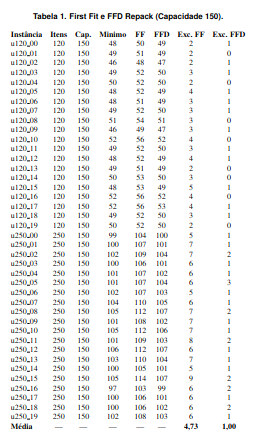
\includegraphics[width=0.67\textwidth]{table-ff.png}

O FFD Repack reduziu o excesso médio de 4,73 para 1,00 bin,
representando uma redução de aproximadamente 78,8\%. Em 8 das 20
instâncias da família \texttt{u120} (u120\_01, u120\_04, u120\_08,
u120\_10, u120\_13, u120\_14, u120\_16 e u120\_19), o algoritmo
atingiu o minimo  conhecido.

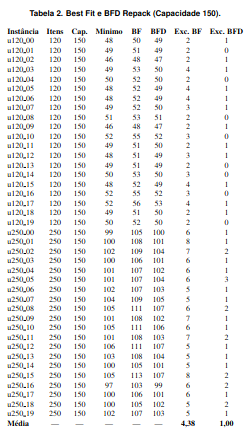
\includegraphics[width=0.65\textwidth]{table-bf.png}

O BFD Repack apresentou excesso médio de 1,00 bin, igual ao observado
para o FFD Repack, com redução de 77,1\% sobre o Best Fit. Esse
resultado sugere que, para a capacidade 150, o remanejamento contribui
para aproximar as soluções do minimo  conhecido,
independentemente da estratégia de encaixe inicial.

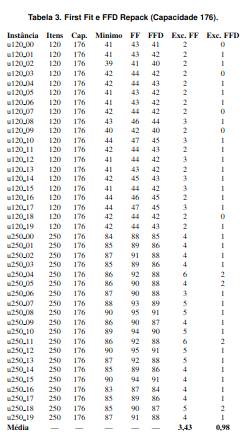
\includegraphics[width=0.65\textwidth]{table-ff-176.png}

Para a capacidade 176, o FFD Repack apresentou excesso médio de
0,98 bin, contra 3,43 do First Fit, o que corresponde a uma redução
de aproximadamente 71,5\%. Em 5 das 20 instâncias da família
\texttt{u120} (u120\_00, u120\_03, u120\_07, u120\_09 e u120\_18), o
algoritmo atingiu o mínimo de bins. Apesar do bom desempenho, o
excesso médio permaneceu ligeiramente superior ao observado para a
capacidade 150 (1,00 contra 0,98 bin), enquanto o gap relativo subiu
de 1,33\% para 1,52\%.

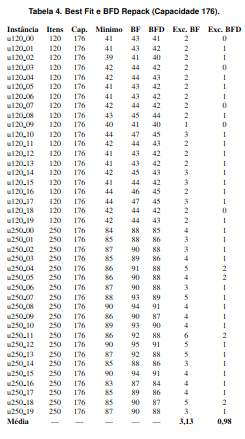
\includegraphics[width=0.75\textwidth]{table-bf-176.png}

Na capacidade 176, o BFD Repack apresentou excesso médio de 0,98 bin,
contra 3,13 do Best Fit, com redução de aproximadamente 68,8\%. Os
resultados são idênticos aos do FFD Repack em todas as instâncias,
confirmando o comportamento observado na capacidade 150: a etapa de
remanejamento domina o efeito da ordenação inicial, e ambos os
algoritmos com remanejamento convergem para as mesmas soluções.

\section{Conclusão}

Os experimentos indicaram que o FFD Repack foi a estratégia com
melhor desempenho geral entre os algoritmos avaliados, considerando
o excesso de bins em relação à minimo  conhecido. Na capacidade
150, o excesso médio foi de 1,00 bin, enquanto na capacidade 176 foi
de 0,98 bin. O BFD Repack apresentou desempenho equivalente em ambas
as capacidades, com os mesmos valores médios. Embora a capacidade 176
tenha produzido soluções com menor número absoluto de bins, o gap
relativo das heurísticas aumentou de 1,33\% para 1,52\%. Como trabalho
futuro, pretende-se avaliar outras estratégias de remanejamento e
investigar o comportamento dos algoritmos em instâncias de maior
porte.

Os resultados também evidenciam que a escolha da capacidade do bin
não é neutra em relação ao desempenho das heurísticas. Ao passar de
150 para 176, o número total de bins na melhor solução conhecida caiu
de 3017 para 2566, mas o gap relativo do FFD Repack subiu de 1,33\%
para 1,52\%. Isso sugere que capacidades maiores, embora reduzam o
desperdício de espaço na solução ótima, tornam o problema
relativamente mais difícil para algoritmos gulosos, pois diminuem a
margem de manobra do remanejamento. Observou-se ainda desempenho
idêntico entre FFD Repack e BFD Repack em ambas as capacidades, o que
indica que a etapa de remanejamento domina o efeito da ordenação
inicial. Por fim, destaca-se que nenhuma instância da família
\texttt{u250} atingiu o minimo em qualquer configuração, sugerindo que
o tamanho da instância influencia diretamente a eficácia das
heurísticas.

\bibliographystyle{sbc}
\bibliography{referencias}

\end{document}
